\subsubsection{Generating an object list}
From the detected coordinates in form of x- and y-coordinates and a detected distance, the distance from the ego-vehicle, velocity, acceleration, angle of the object and angular velocity, can be calculated. For the calculation previous values are stored and assigned to an ID. With the proportionality of the object distance from the vertical centerline and the camera angle, the script scales in metric distance.

%\begin{equation}
%D_{Center} = Y_{Pixel} - \frac{FO_{Horizontal}}{2}
%\label{test}
%\end{equation}

\begin{equation}
		d_{Pixel} = y_{Pixel} -  \frac{w_{Pixel}}{2}\\	
\end{equation}
\begin{table}[!h]
	\begin{center}
		\begin{tabular}{l c l}
			$d_{Pixel}$ & = & distance from centerline to object\\
			$y_{Pixel}$ & = &  y-coordinates of the object\\
			$w_{Pixel}$ & = & pixel format of the video horizontal\\
		\end{tabular}
	\end{center}
\end{table}



This formula divides the image into two segments (left and right segment) and calculates the distance of the object to this center axis.

\begin{equation}
k_{angle}  = \frac{d_{Pixel}}{w_{Segment,Pixel}}
\end{equation}
\begin{table}[!h]
	\begin{center}
		\begin{tabular}{l c l}
			$k_{angle}$ & = & proportionality factor for distance and angle\\
			$w_{Segment,Pixel}$ & = &  pixel width of segment\\
		\end{tabular}
	\end{center}
\end{table}

Here is a factor calculated, which corresponds to a value of -1...0 or 0...1. This indicates, which factor of the total segment width, the object is located.

\begin{equation}
\phi = k_{angle} * \alpha_{Segment}
\end{equation}
\begin{table}[!h]
	\begin{center}
		\begin{tabular}{l c l}
			$\phi$ & = & angle from centerline to object\\
			$\alpha_{Segment}$ & = &  angle of view of a Segment = \ang{45}\\
		\end{tabular}
	\end{center}
\end{table}

The angle of view from the camera, which corresponds to \ang{90}, is used. In relation to a segment, it would be \ang{45}. This is calculated with the factor, to get an angle related to the vertical axis.

\begin{figure}[h]
	\centering
	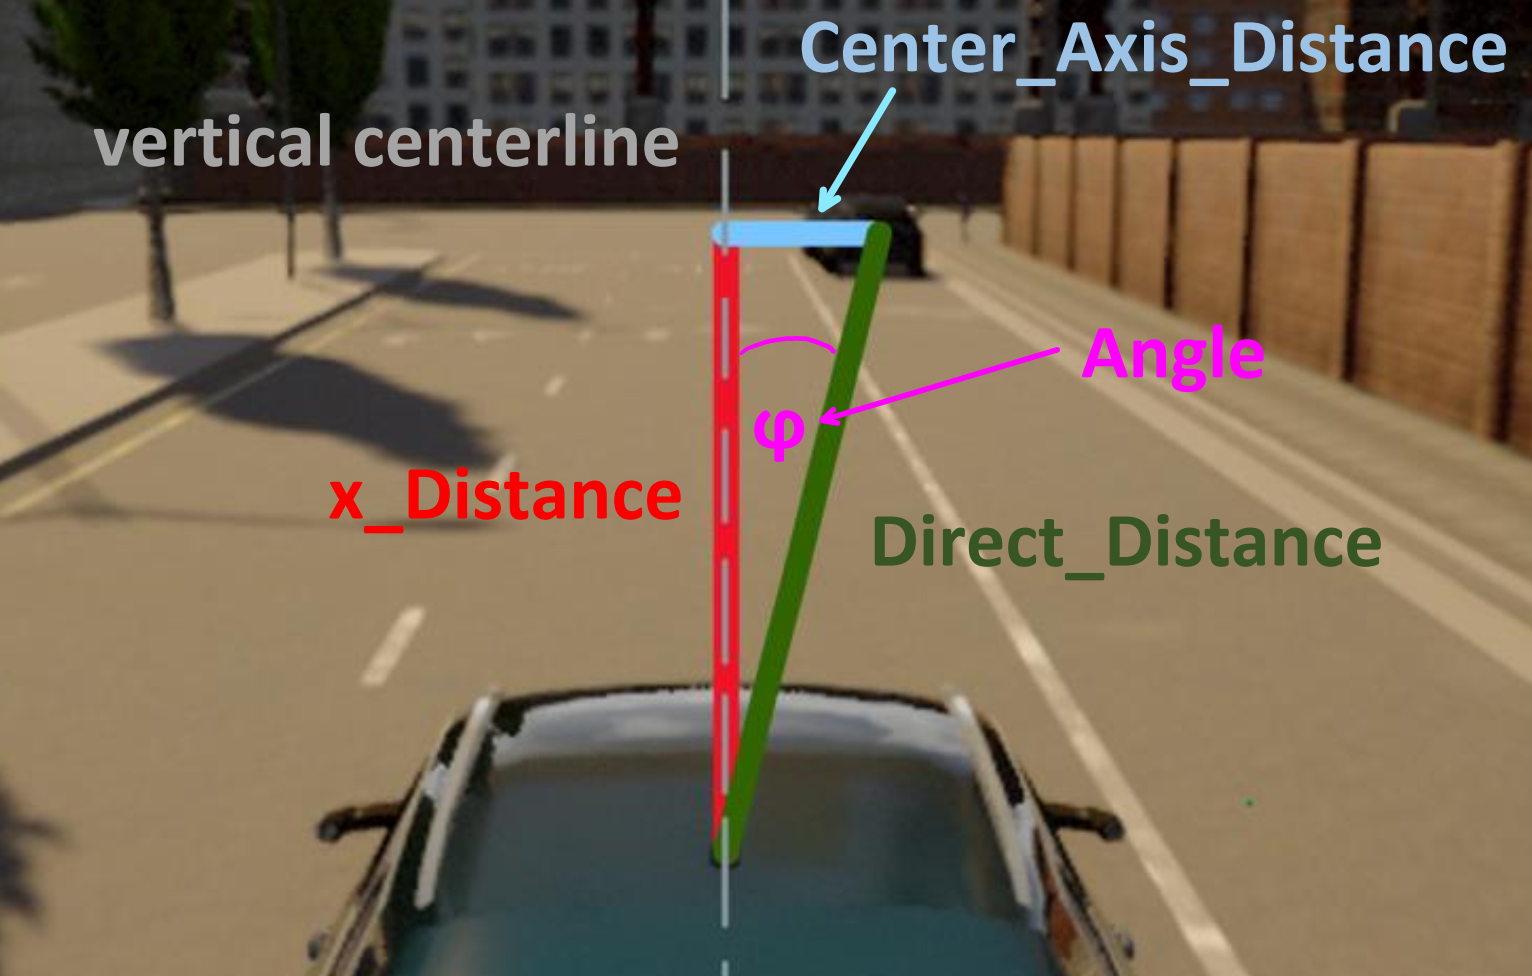
\includegraphics[width=0.4\textwidth]{calc_angle.png}
	\caption{Calculation of angle}
	\label{fig:anglecalculation}
\end{figure}

By using the angle and the direct distance, the trigonometric theorems can be used to calculate the x- and y-distance in meters, which are the basis for the velocity- , acceleration- , angle- , and angular velocity-calculation. The object attributes are stored over several frames to calculate time-dependent values. Velocity is calculated by the change of the x- and y-distances, the acceleration, by changing the x- and y-velocities. The angle with the Velocity in x- and y-direction and the angular velocity is calculated by time changing angles. The calculated values are related to the ego-vehicle.
The dimensioning is based on the same formulas. The formulas above are used to calculate an angle. This angle can be used, to calculate a distance in meters from the center vertical axis, for the position of the vehicle on the y-axis.

\begin{equation}
	y = h_{direct} * sin(\frac{\phi * \pi}{180})
\end{equation}
\begin{table}[!h]
	\begin{center}
		\begin{tabular}{l c l}
			$y$ & = & distance from centerline to object in meters\\
			$h_{direct}$ & = &  direct distance to object in meters\\
		\end{tabular}
	\end{center}
\end{table}

After calculating the distance of the object to the center axis of the image, it is divided by the pixel distance of the object according to the center axis. This gives a meter per pixel value, to convert the detected object dimensions in pixels, to meter.

\begin{equation}
	k_{MpP} = \frac{y}{d_{Pixel}}
\end{equation}
\begin{table}[!h]
	\begin{center}
		\begin{tabular}{l c l}
			$k_{MpP}$ & = & factor meter per pixel for scaling\\
		\end{tabular}
	\end{center}
\end{table}

Via the \ac{ROS} Framework, the required data such as geometry, probability, \ac{ID} of the object etc. are transferred via a node in form of a message. A topic receives this message for further processing of the data in \ac{RVIZ} (\ac{ROS}).

\begin{figure}[h]
	\centering
	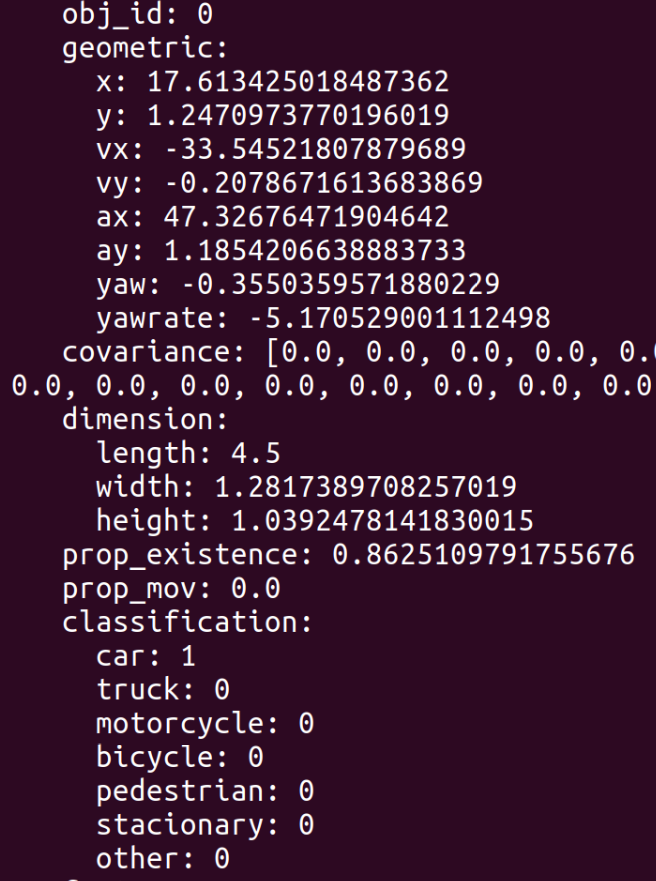
\includegraphics[width=0.3\textwidth]{images/objlist_output.png}
	\caption{Generated Object List}
	\label{fig:ros_outout}
\end{figure}